\documentclass[aspectratio = 169]{beamer}
%======================================================================================================================%
% Preamble
\usepackage[
    backend = biber,
    style = apa,
    citestyle = authoryear-comp,
    sorting = ydnt,
    mincitenames = 1,
    maxcitenames = 2,
    uniquelist = minyear
]{biblatex}
\addbibresource{emissions.bib}
\AtBeginBibliography{\small}

\usepackage{hyperref}
\hypersetup{colorlinks = true, citecolor = blue, linkcolor = blue, urlcolor = blue, hypertexnames = true}
\newcommand{\shortlink}[1]{\href{https://www.#1}{\texttt{#1}}}

\DeclareCiteCommand{\cite} % Ensures author-year hyperlink applies to \cite
{\usebibmacro{prenote}}
{\usebibmacro{citeindex}%
\printtext[bibhyperref]{\usebibmacro{cite}}}
{\multicitedelim}
{\usebibmacro{postnote}}

\DeclareCiteCommand{\parencite}[\mkbibparens] % Ensures author-year hyperlink applies to \parencite
{\usebibmacro{prenote}}
{\usebibmacro{citeindex}%
\printtext[bibhyperref]{\usebibmacro{cite}}}
{\multicitedelim}
{\usebibmacro{postnote}}

\DeclareCiteCommand{\cite} % Ensures that year appears in parentheses
{\usebibmacro{prenote}}
{\usebibmacro{citeindex}%
\printtext[bibhyperref]{\printnames{labelname} \mkbibparens{\printfield{year}}}}
{\multicitedelim}
{\usebibmacro{postnote}}

% Packages
\usepackage{graphicx} % Required for inserting images
\usepackage{amsmath}
\usepackage{amsfonts}
\usepackage{mathrsfs}
\usepackage{array}
\usepackage{booktabs}
\usepackage{float}
\usepackage{textcomp}
\usepackage{color}
\usepackage{stmaryrd}
%\usepackage{blkarray}
%======================================================================================================================%
% Themes
%\usetheme{madrid}
%\usetheme{Warsaw}
%\usetheme{Boadilla}
\usetheme[progressbar = frametitle]{metropolis}
\setbeamertemplate{frame numbering}[fraction]
\metroset{background = dark}

\definecolor{primary}{RGB}{2, 25, 232}
\setbeamercolor{palette primary}{bg = white, fg = black}
\setbeamercolor{background canvas}{parent = palette primary}
\setbeamercolor{normal text}{fg = black}
\setbeamercolor{progress bar}{use = palette primary, fg = primary}

%\setbeamercovered{transparent}
%%%%%%%%%%%%%%%%%%%%%%%%%%%%%%%%%%%%%%%%%%%%%%%%%%%%%%%%%%%%%%%%%%%%%%%%%%%%%%%%%%%%%%%%%%%%%%%%%%%%%%%%%
% Title and Authors
\title[]{Unforeseen Minimum Wage Consequences}

\author[Ekeocha]{
    D.O.~Ekeocha\inst{1}
%    \and
%    D.F. ~Giuseppe\inst{1}
%    \and
%    J. ~Lonsky\inst{1}
}
\institute[]{
    \inst{1}
    University of Liverpool Management School
}
\date{\today}
%======================================================================================================================%
% Document
\begin{document}
    \maketitle

    \begin{frame}{Outline}
        \tableofcontents
    \end{frame}


    \section{Motivation}\label{sec:motivation}
    \begin{frame}{Motivation}
        \begin{itemize}
            \item<1-> Wages and labour cost~\parencite{coviello2022minimum, alexandre2022minimum, gopalan2021state}
            \item<2-> Employment~\parencite{brown1999minimum, neumark1992employment, card2000minimum, cengiz2019effect, dustmann2022reallocation, neumark2019econometrics}
            \item<3-> Consumers via higher prices~\parencite{harasztosi2019pays}
            \item<4-> Pollution?~\parencite{zhang2023unintended}
        \end{itemize}
    \end{frame}

    \begin{frame}[shrink = 30]{Distribution of Total Toxic Releases Intensity}
        \begin{figure}[H]
    \centering
    \includegraphics[width = 0.8\textwidth]{fig_releases_distribution}
    \caption{Distribution of Total Onsite Releases Intensity across Manufacturing Industries}
    \label{fig:releases-distribution}
\end{figure}
    \end{frame}

    \begin{frame}[shrink = 30]{Distribution of Air Emissions Intensity}
        \begin{figure}[H]
    \centering
    \includegraphics[width = 0.8\textwidth]{C:/Users/david/OneDrive/Documents/ULMS/PhD/Thesis/chapter3/src/climate_change/latex/fig_air_emissions_distribution_naics}
    \caption{Distribution of Total Onsite Air Emissions Intensity across Manufacturing Industries}
    \label{fig:air-emissions-distribution-naics}
\end{figure}
    \end{frame}

    \begin{frame}{Leading Questions}
        \begin{enumerate}
            \item Is this increased cost-burden due to higher MW passed to the environment, in terms of higher pollution emissions per $\$100m$ units of output?
            \item Is the environmental impact of raising MW heterogeneous across cohorts and manufacturing industries?
        \end{enumerate}
    \end{frame}


    \section{Data and Identification Strategy}\label{sec:data-and-identification-strategy}
    \begin{frame}{Border States and Counties}
        %\usepackage{booktabs}
\begin{table}[H]
    \centering
    \caption{Exogenous State-level MW Adjustments}
    \label{tab:states-mw-adjustments-t-and-c}
    \resizebox{\columnwidth}{!}{%
        \begin{tabular}{lrrrrrrlrr}
            \toprule\toprule
            treated states & MW $\Delta$ year & MW $\Delta$ amount & $\sum_{1}^{2}\Delta MW$ & total MW $\Delta$ amount & start MW & end MW & control states & \# of border counties (T) & \# of border counties (C) \\ \midrule\midrule
            MN             & 2014             & 1.85               & 1.50                    & 3.35                     & 6.16     & 9.51   & (IA, ND, WI)   & 42                        & 54                        \\
            MA             & 2015             & 1.00               & 2.00                    & 3.00                     & 8.00     & 11.00  & (NH)           & 8                         & 6                         \\
            CA             & 2014             & 1.00               & 1.50                    & 2.50                     & 8.00     & 10.50  & (NV)           & 10                        & 11                        \\
            NY             & 2014             & 0.75               & 1.70                    & 2.45                     & 7.25     & 9.70   & (PA)           & 27                        & 16                        \\
            AR             & 2015             & 1.25               & 1.00                    & 2.25                     & 6.25     & 8.50   & (OK, TX)       & 19                        & 12                        \\
            MD             & 2015             & 1.00               & 1.00                    & 2.00                     & 7.25     & 9.25   & (PA, VA)       & 21                        & 39                        \\
            NE             & 2015             & 0.75               & 1.00                    & 1.75                     & 7.25     & 9.00   & (IA, KS, WY)   & 28                        & 24                        \\
            ME             & 2017             & 1.50               & 0.00                    & 1.50                     & 7.50     & 9.00   & (NH)           & 5                         & 7                         \\
            MI             & 2014             & 0.75               & 0.75                    & 1.50                     & 7.40     & 8.90   & (IL, IN, WI)   & 32                        & 39                        \\
            WV             & 2015             & 0.75               & 0.75                    & 1.50                     & 7.25     & 8.75   & (KY, PA, VA)   & 32                        & 28                        \\
            SD             & 2015             & 1.25               & 0.15                    & 1.40                     & 7.25     & 8.65   & (IA, ND, WY)   & 27                        & 19                        \\
            NJ             & 2014             & 1.00               & 0.19                    & 1.19                     & 7.25     & 8.44   & (PA)           & 16                        & 13                        \\
            DE             & 2014             & 0.50               & 0.50                    & 1.00                     & 7.25     & 8.25   & (PA)           & 5                         & 6                         \\ \bottomrule\bottomrule
        \end{tabular}
    }
    \begin{minipage}{17.5cm}
        \vspace{0.01in}
        \tiny NOTES: This table summarizes the exogenous state-level MW changes from $2012$ to $2017$. There are thirteen $(13)$ treated and $(14)$ control states. The definition of treated and control states is given in sub-section~\ref{subsec:selecting-the-treated-and-control-states}. MW $\Delta$ year represents the year in which a treated state first raised its MW. MW $\Delta$ amount corresponds to the first MW raised amount for that year. $\sum_{1}^{2}\Delta MW$ denotes the sum of any post-two-year MW raises after the first initial raise. Total MW $\Delta$ amount corresponds to the total MW raised amount till the end of the sample. Start (End) is the MW at the start (end) of the sample. Control states are the set of control states for each treated states. These states never raised MW between $2012$ and $2017$. \# of border counties (T) is the number of counties in a treated state that border at least one county in a control state. And \# of border counties (C) is the number of counties in a control state that border at least one county in a treated state. * means not used in the POTWs sample.
    \end{minipage}
\end{table}

        \hypertarget{Border States}{}
        \hyperlink{fig:border-state-map}{\beamergotobutton{Border States}}
        \hypertarget{Border Counties}{}
        \hyperlink{fig:border-county-map}{\beamergotobutton{Border Counties}}
    \end{frame}

    \begin{frame}{Data}
        \begin{itemize}
            \item EPA: TRI facility information
            \item NBER-CES: Industry Information, Costs, Employment and Output
            \item QCEW: Number of establishments in each county
            \item BEA and BLS-CPI: County-level GDP and CPI
            \item US Shapefiles
            \item Unbalance panel of facilities, chemicals, counties, and states---$(2011-2017)$
        \end{itemize}
        \hypertarget{Summary Table}{}
        \hyperlink{tab:summary-table}{\beamergotobutton{Summary Table}}
        \hypertarget{Balance Test Counties}{}
        \hyperlink{tab:balance-test-counties}{\beamergotobutton{Balance Test Counties}}
        \hypertarget{Balance Test States}{}
        \hyperlink{tab:balance-test-states}{\beamergotobutton{Balance Test States}}
    \end{frame}


    \section{Baseline Results}\label{sec:baseline-results}
    \begin{frame}[shrink = 30]{Higher Industry Costs}
        \begin{figure}[H]
    \centering
    \includegraphics[width=1\textwidth,keepaspectratio]{fig_sdid_industry_costs}
    \caption{Manufacturing Industry Costs}
    \label{fig:baseline-manufacturing-industry-costs}
    \begin{minipage}{14cm}
        \vspace{0.05in}
        NOTES: The event study model of equation~\ref{eq:baseline-wages} is $C_{i,cp,t} = \sum_{{e = -3},{e \neq -1}}^{3} \beta Treated_{s,t}^e = \textbf{1}[t - G_{s,t}] + \delta X_{v,c,t-1} + \omega P_{f,t} + \lambda_{t} + \sigma_{c} + \phi_{cp} + \zeta_{cp,t} + \epsilon_{i,cp,t}$. Standard errors are clustered at the state level. de Chaisemartin and D'Haultfoeuille Decomposition: $\sum dCDH_{ATTs}^{weights(+)} = 1$ and $\sum dCDH_{ATTs}^{weights(-)} = 0$.
    \end{minipage}
\end{figure}
        \hypertarget{Industry Costs}{}
        \hyperlink{tab:baseline-costs}{\beamergotobutton{Costs}}
    \end{frame}

    \begin{frame}[shrink = 30]{Employment and Hours}
        \begin{figure}[H]
    \centering
    \includegraphics[width=1\textwidth, keepaspectratio]{fig_sdid_emp_hours}
    \caption{Industry Employment and Production Workers Hours}
    \label{fig:baseline-employment-hours}
    \begin{minipage}{14cm}
        \vspace{0.05in}
        NOTES: The event study model of equation~\ref{eq:baseline-emp-hours} is $E_{i,cp,t} = \sum_{{e = -3},{e \neq -1}}^{3} \beta Treated_{s,t}^e = \textbf{1}[t - G_{s,t}] + \delta X_{v,c,t-1} + \omega F_{f,t} + \lambda_{t} + \sigma_{c} + \phi_{cp} + \zeta_{cp,t} + \epsilon_{i,cp,t}$. Standard errors are clustered at the state level. de Chaisemartin and D'Haultfoeuille Decomposition: $\sum dCDH_{ATTs}^{weights(+)} = 1$ and $\sum dCDH_{ATTs}^{weights(-)} = 0$.
    \end{minipage}
\end{figure}
        \hypertarget{Employment and Hours}{}
        \hyperlink{tab:baseline-employment-hours}{\beamergotobutton{Employment}}
        \hypertarget{Cross-County Worker Mobility}{}
        \hyperlink{tab:baseline-worker-mobility}{\beamergotobutton{Worker Mobility}}
    \end{frame}

    \begin{frame}[shrink = 30]{Outputs}
        \begin{figure}[H]
    \centering
    \includegraphics[width=1\textwidth, keepaspectratio]{C:/Users/david/OneDrive/Documents/ULMS/PhD/Thesis/chapter3/src/climate_change/latex/fig_sdid_output}
    \caption{Manufacturing Industry Output: Output per Hour and Output per Worker}
    \label{fig:baseline-industry-output}
    \begin{minipage}{\columnwidth}
        \vspace{0.05in}
        \tiny NOTES: The event study model of equation~\ref{eq:baseline-wages} is $Y_{i,cp,t} = \sum_{{e = -3},{e \neq -1}}^{3} \beta Treated_{s,t}^e = \textbf{1}[t - G_{s,t}] + \delta X_{v,c,t-1} + \omega F_{f,t} + \lambda_{t} + \sigma_{c} + \phi_{cp} + \zeta_{cp,t} + \epsilon_{i,cp,t}$. Standard errors are clustered at the state level. de Chaisemartin and D'Haultfoeuille Decomposition: $\sum dCDH_{ATTs}^{weights(+)} = 1$ and $\sum dCDH_{ATTs}^{weights(-)} = 0$.
    \end{minipage}
\end{figure}
        \hypertarget{Outputs}{}
        \hyperlink{tab:baseline-outputs}{\beamergotobutton{Output}}
    \end{frame}


    \section{Does MW Induce Unintended Consequences?}\label{sec:consequences}
    \begin{frame}{Onsite Toxic Releases Intensity}
        \begin{figure}[H]
    \centering
    \includegraphics[width=1\textwidth, height=0.5\textheight,keepaspectratio]{fig_sdid_total_releases_onsite_int}
    \caption{Total Onsite Releases Intensity}
    \label{fig:baseline-total-onsite-releases-intensity}
    \begin{minipage}{18cm}
        \vspace{0.05in}
        NOTES: The event study model of equation~\ref{eq:baseline-total-onsite-releases-intensity} is $P_{f,cp,c,t} = \sum_{{e = -3},{e \neq -1}}^{3} \beta Treated_{s,t}^e + \delta X_{v,c,t-1} + \omega F_{f,t} + \lambda_{t} + \gamma_{f} + \phi_{cp} + \zeta_{c} + \eta_{c,t} + \varepsilon_{f,cp,c,t}$. Three-way clustered robust standard errors are reported in parentheses, and clustered at the toxic chemical, industry and state levels. The test for the presence of pre-trends shows and F-statistic of $0.1461$ $(0.9296)$, p-value (in parentheses) using F-Statistic $(\chi^2): \sum_{-3}^{-2} \beta_{e} = 0$. de Chaisemartin and D'Haultfoeuille Decomposition: $\sum dCDH_{ATTs}^{weights(+)} = 1$ and $\sum dCDH_{ATTs}^{weights(-)} = 0$.
    \end{minipage}
\end{figure}
        \hypertarget{Toxic Releases Intensity}{}
        \hyperlink{tab:toxic-releases-intensity}{\beamergotobutton{Toxic Releases Intensity}}
    \end{frame}

    \begin{frame}[shrink = 10]{Onsite Toxic Air Emissions Intensity}
        \begin{figure}[H]
    \centering
    \includegraphics[width=1\textwidth, height=0.5\textheight,keepaspectratio]{C:/Users/david/OneDrive/Documents/ULMS/PhD/Thesis/chapter3/src/climate_change/latex/fig_sdid_onsite_air_emissions_int}
    \caption{Total Onsite Releases Intensity}
    \label{fig:baseline-onsite-air-emission-intensity}
    \begin{minipage}{\columnwidth}
        \vspace{0.05in}
        \tiny NOTES: The event study model of equation~\ref{eq:baseline-onsite-air-emission-intensity} is $A_{f,cp,c,t} = \sum_{{e = -3},{e \neq -1}}^{3} \beta Treated_{s,t}^e + \omega F_{f,t} + \lambda_{t} + \gamma_{f} + \phi_{cp} + \zeta_{c} + \eta_{c,t} + \theta_{cp,t} + \varepsilon_{f,cp,c,t}$. Three-way clustered robust standard errors are reported in parentheses, and clustered at the toxic chemical, industry and state levels. de Chaisemartin and D'Haultfoeuille Decomposition: $\sum dCDH_{ATTs}^{weights(+)} = 1$ and $\sum dCDH_{ATTs}^{weights(-)} = 0$.
    \end{minipage}
\end{figure}
        \hypertarget{Toxic Air Emissions Intensity}{}
        \hyperlink{tab:toxic-air-emissions-intensity}{\beamergotobutton{Toxic Air Emissions Intensity}}
    \end{frame}

    \begin{frame}[shrink = 20]{Onsite Water Discharge Intensity}
        \begin{figure}[H]
    \centering
    \includegraphics[width=1\textwidth, height=0.5\textheight,keepaspectratio]{C:/Users/david/OneDrive/Documents/ULMS/PhD/Thesis/chapter3/src/climate_change/latex/fig_sdid_onsite_water_discharge_int}
    \caption{Total Onsite Releases Intensity}
    \label{fig:baseline-onsite-water-discharge-intensity}
    \begin{minipage}{18cm}
        \vspace{0.05in}
        \tiny NOTES: The event study model of equation~\ref{eq:baseline-onsite-water-discharge-intensity} is $W_{f,cp,c,t} = \sum_{{e = -3},{e \neq -1}}^{3} \beta Treated_{s,t}^e + \delta X_{v,c,t-1} + \omega F_{f,t} + \lambda_{t} + \gamma_{f} + \phi_{cp} + \zeta_{c} + \eta_{c,t} + \theta_{cp,t} + \varepsilon_{f,cp,c,t}$. Three-way clustered robust standard errors are reported in parentheses, and clustered at the toxic chemical, industry and state levels. de Chaisemartin and D'Haultfoeuille Decomposition: $\sum dCDH_{ATTs}^{weights(+)} = 1$ and $\sum dCDH_{ATTs}^{weights(-)} = 0$.
    \end{minipage}
\end{figure}
        \hypertarget{Toxic Water Discharge Intensity}{}
        \hyperlink{tab:toxic-water-discharge-intensity}{\beamergotobutton{Toxic Water Discharge Intensity}}
    \end{frame}

    \begin{frame}[shrink = 30]{Differential Impacts}
        % Please add the following required packages to your document preamble:
% \usepackage{booktabs}
% \usepackage{graphicx}
\begin{table}[H]
    \centering
    \caption{Onsite Releases Intensity given Highest Emitting Manufacturing Industries}
    \label{tab:heterogeneous-onsite-releases-int-heis}
    \resizebox{\columnwidth}{!}{%
        \begin{tabular}{@{}llllllll@{}}
            \toprule\toprule
            Onsite releases intensity (log) & total     & air emissions & point air & fugitive air & water discharge & land releases & surface impoundment \\ \midrule
            $Treated^{e} \cdot D$           & 0.360***  & 0.224***      & 0.032     & 0.235***     & 0.094           & 0.002         & -0.011**            \\
            & (0.116)   & (0.077)       & (0.066)   & (0.067)      & (0.087)         & (0.019)       & (0.005)             \\
            $Treated^{e}$                   & 0.020     & 0.023         & 0.048     & -0.011       & 0.007           & 0.007         & 0.021**             \\
            & (0.039)   & (0.039)       & (0.036)   & (0.030)      & (0.011)         & (0.013)       & (0.010)             \\
            cohort 2014 $\cdot D$           & 0.350***  & 0.305***      & 0.259**   & 0.077        & -0.079          & 0.041         & -0.011**            \\
            & (0.113)   & (0.114)       & (0.107)   & (0.077)      & (0.067)         & (0.044)       & (0.005)             \\
            cohort 2015 $\cdot D$           & 0.369***  & 0.149**       & -0.178*   & 0.381***     & 0.254**         & -0.034        & -0.012              \\
            & (0.141)   & (0.069)       & (0.091)   & (0.090)      & (0.122)         & (0.021)       & (0.007)             \\
            cohort 2017 $\cdot D$           & 0.052     & 0.032         & 0.166     & 0.145        & 0.033           & 0.025         & -0.002              \\
            & (0.174)   & (0.179)       & (0.141)   & (0.142)      & (0.091)         & (0.025)       & (0.009)             \\
            controls                        & Yes       & Yes           & Yes       & Yes          & Yes             & Yes           & Yes                 \\
            year FE                         & Yes       & Yes           & Yes       & Yes          & Yes             & Yes           & Yes                 \\
            facility FE                     & Yes       & Yes           & Yes       & Yes          & Yes             & Yes           & Yes                 \\
            border-county FE                & Yes       & Yes           & Yes       & Yes          & Yes             & Yes           & Yes                 \\
            toxic chemical FE               & Yes       & Yes           & Yes       & Yes          & Yes             & Yes           & Yes                 \\
            toxic chemical LTs              & Yes       & Yes           & Yes       & Yes          & Yes             & Yes           & Yes                 \\\midrule
            Observations                    & 1,893,689 & 1,893,689     & 1,893,689 & 1,893,689    & 1,893,689       & 1,893,689     & 1,893,689           \\
            $R^2$                           & 0.720     & 0.739         & 0.712     & 0.661        & 0.585           & 0.501         & 0.127               \\ \bottomrule \bottomrule
        \end{tabular}%
    }
    \begin{minipage}{\columnwidth}
        \vspace{0.05in}
        \tiny NOTES: These results are obtained from estimating this equation: $P_{f,cp,c,t}^{heis} = \beta (Treated^{e} \cdot D)_{f,s,t} + \psi (Treated^{e})_{s,t} + \vartheta (Treated \cdot D)_{f,s,t} + \mu (Post \cdot D)_{f,s,t} + \tau Treated_{s,t} + \rho D_{f,s,t} + \alpha Post_{t} + \delta X_{v,c,t-1} + \omega F_{f,t} + \lambda_{t} + \gamma_{f} + \phi_{cp} + \zeta_{c} + \eta_{c,t} + \varepsilon_{f,cp,c,t}$. Three-way clustered robust standard errors are reported in parentheses, and clustered at the toxic chemical, industry and state levels. ***, **, and * denote significance levels at the less than $1\%$, $5\%$ and $10\%$, respectively.
    \end{minipage}
\end{table}
        \hypertarget{Onsite Releases Intensities}{}
        \hyperlink{fig:heterogeneous-onsite-releases-int-heis}{\beamergotobutton{Onsite Releases Intensities}}
    \end{frame}


    \section{Mechanisms}\label{sec:mechanisms}
    \begin{frame}{Waste Management}
        \begin{enumerate}
            \item Declining thermal treatments
            \item Declining kiln energy recovery methods
            \item Declining recycling of chemical wastes for reuse in the production process
        \end{enumerate}
        \hypertarget{Mechanism Waste Management}{}
        \hyperlink{tab:mechanism-waste-management}{\beamergotobutton{Waste Management}}
    \end{frame}

    \begin{frame}{Source Reduction Activities}
        \begin{enumerate}
            \item Substituting organic solvents (-ve)
            \item Manufacturing aid and ancillary chemicals (-ve)
            \item Substituting clean fuels (-ve) and higher energy intensity (+ve)
            \item Product modifications (-ve)
            \item Poor material handling, monitoring, and no training (-ve)
            \item Optimised efficiency of production processes (+ve)
            \item New green technologies (+ve)
            \item Green R and D projects (+ve)
        \end{enumerate}
        \hypertarget{Mechanism Source Reduction}{}
        \hyperlink{tab:mechanism-source-reduction}{\beamergotobutton{Source Reduction}}
        \hypertarget{Mechanism Material Products}{}
        \hyperlink{tab:mechanism-material-products-submod}{\beamergotobutton{Material Products}}
        \hypertarget{Mechanism Process}{}
        \hyperlink{tab:mechanism-process}{\beamergotobutton{Process}}
        \hypertarget{Mechanism Inventory Operations}{}
        \hyperlink{tab:mechanism-inventory-operations}{\beamergotobutton{Inventory Operations}}
    \end{frame}


    \section{Concluding Remarks}\label{sec:concluding-remarks}
    \begin{frame}{Concluding Remarks}
        \begin{itemize}
            \item Heterogeneous environmental consequences of raising MW
            \item Mostly dominated in highest emitting industries
            \item Consequential even in highly regulated domains---Point sources
        \end{itemize}
    \end{frame}
%======================================================================================================================%

%    \section{Theoretical Analysis}\label{sec:theoretical-analysis}
%    \begin{frame}{Theoretical Analysis}
%        \begin{itemize}
%            \item There are two competing hypotheses: \textbf{The induced technology change effect and the crowding-out effect.}
%        \end{itemize}
%
%        Unintended consequences of a raising minimum wage is an empirical question!
%
%    \end{frame}
%
%
%    \section{Data \& Identification Strategy}\label{sec:data-and-identification}
%    \begin{frame}{Data}
%        \begin{itemize}
%            \item MW data---county level from $1997$ to $2009$ from Ministry of Human Resources and Social Security.
%            \item Pollutant emissions data (chemical oxide demand and sulphur oxide) $1998$ to $2009$---firm level from China's Environmental Statistics Database (CESD) and China's Industrial Enterprise Database (CIED).
%            \item Green innovation (green patents) from State's Intellectual Property Office.
%            \item Regional macroeconomic variables (GDP and local employment)---county and city level from the Chinese Statistical Year Book.
%        \end{itemize}
%    \end{frame}
%
%    \begin{frame}{Summary Statistics}
%        \begin{figure}
%            \centering
%            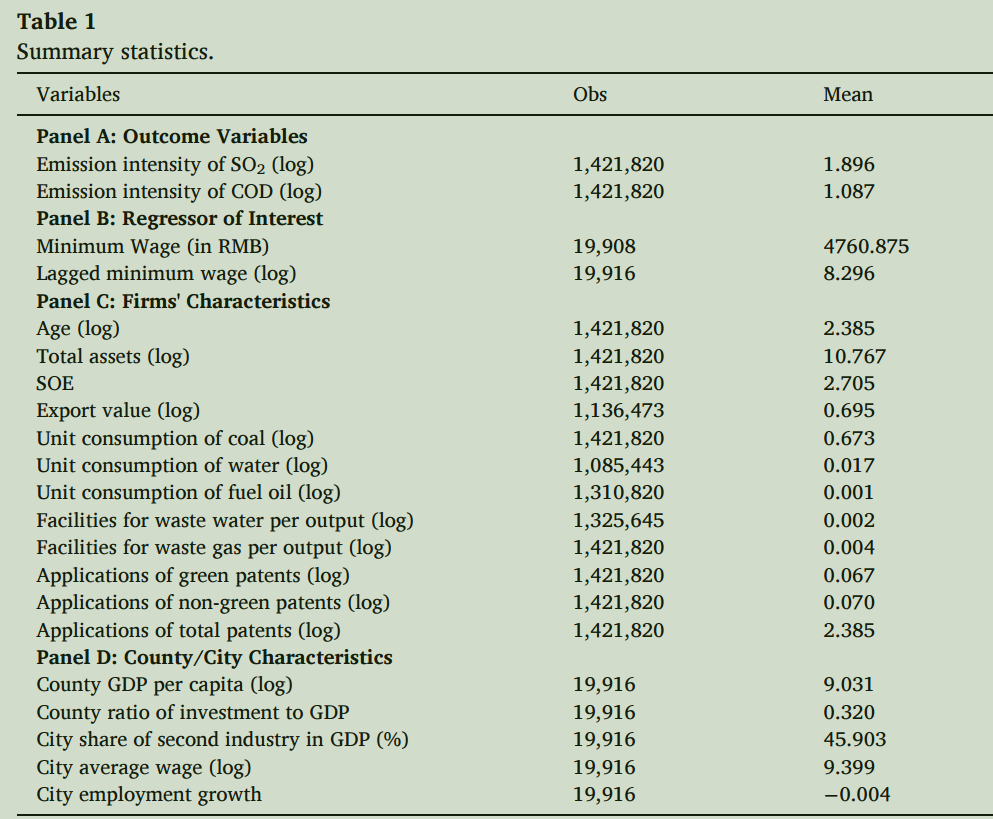
\includegraphics[width = 0.6\textwidth, height = 0.8\textheight]{climate_change/beamer/sumstat}
%%                \caption{Evolution of MW in Chinese Counties}
%            \label{fig:sumstat}
%        \end{figure}
%    \end{frame}
%
%    \begin{frame}{Identification Strategy---County Border Discontinuity}
%        \begin{itemize}
%            \item They leveraged discontinuity in MW policy between adjacent Chinese county pairs at the border~\parencite{dube2010minimum}.
%            \item Average MW growth is $9.5\%$.
%            \item County pairs must share the same border and range between $50km$, $75km$ and $100km$ away from the border.
%            \item Final sample $1,183,702$, $1,214,918$ and $1,217,919$, respectively.
%            \item And $89,248$ distinct firms.
%        \end{itemize}
%
%    \end{frame}
%
%    \begin{frame}{County Border Discontinuity}
%        \begin{columns}
%            \column{0.5\textwidth}
%            \begin{figure}
%                \centering
%                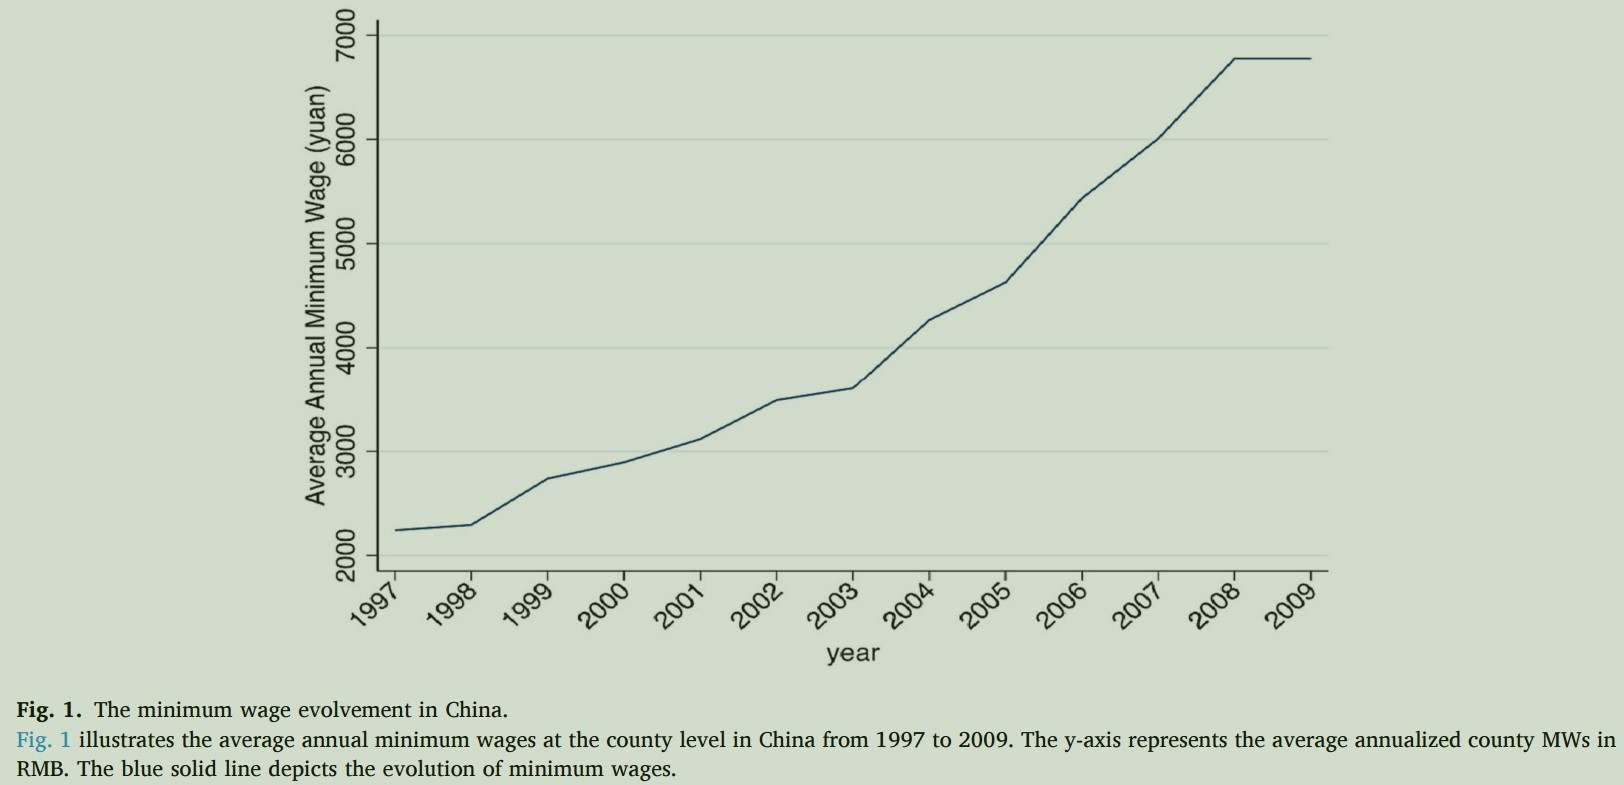
\includegraphics[width = \textwidth, height = 0.6\textheight]{climate_change/beamer/wd}
%%                \caption{Evolution of MW in Chinese Counties}
%                \label{fig:chinese-mw1}
%            \end{figure}
%
%            \column{0.5\textwidth}
%            \begin{figure}
%                \centering
%                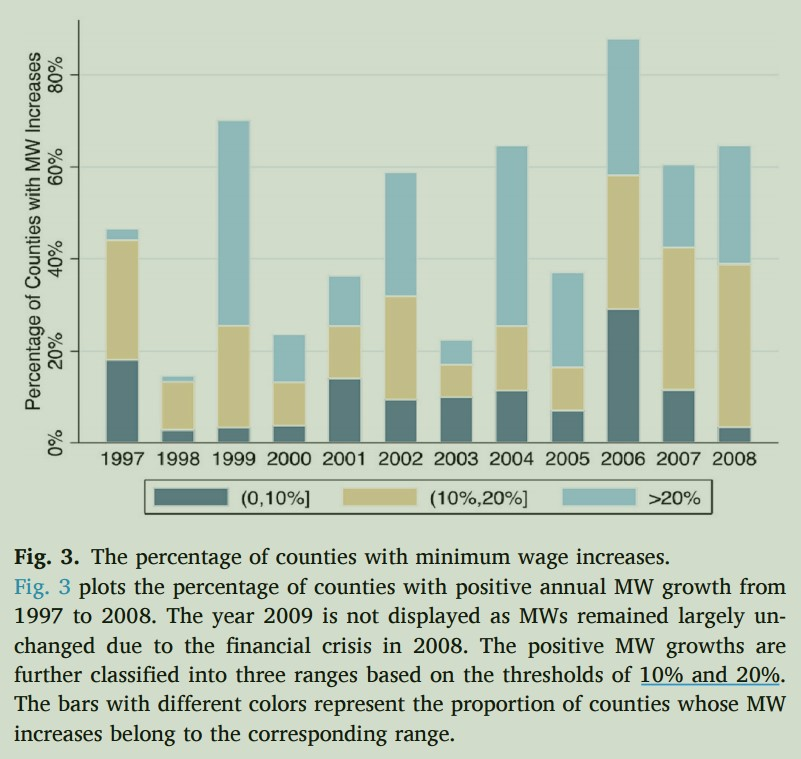
\includegraphics[width = \textwidth, height = 0.7\textheight]{climate_change/beamer/wd2}
%%                \caption{Evolution of MW in Chinese Counties}
%                \label{fig:chinese-mw2}
%            \end{figure}
%        \end{columns}
%    \end{frame}

%    \begin{frame}[shrink = 25]{Summary Statistics}
%        \input{energy_effects/results/tables/cov.grid.nt.sum.stat}
%    \end{frame}
%=======================================================================================================================%
    \begin{frame}[allowframebreaks, noframenumbering]
%        \frametitle{Appendix}
        \hypertarget{fig:border-states}{}
        \begin{figure}
            \centering
            \includegraphics[width=0.7\textwidth,height=0.65\textheight]{fig_border_state_map}
            \caption{Border States}
            \label{fig:border-state-map}
        \end{figure}
        \hyperlink{Border States}{\beamergotobutton{Return}}
        \fontsize{9}{11}\selectfont
    \end{frame}

    \begin{frame}[allowframebreaks, noframenumbering]
%        \frametitle{Appendix}
        \hypertarget{fig:border-counties}{}
        \begin{figure}
            \centering
            \includegraphics[width=0.7\textwidth,height=0.65\textheight]{fig_border_county_map}
            \caption{Border Counties}
            \label{fig:border-county-map}
        \end{figure}
        \hyperlink{Border Counties}{\beamergotobutton{Return}}
        \fontsize{9}{11}\selectfont
    \end{frame}

    \begin{frame}[shrink = 1, allowframebreaks, noframenumbering]
        \hypertarget{tab:summary-table}{}
        \begin{table}[H]
    \centering
    \caption{Summary Statistics (Onsite)}
    \label{tab:sumstat-onsite}
    \resizebox{\textwidth}{!}{
        \begin{tabular}{lrrrrr}
            \toprule \toprule
            Variable                                                & Obs     & Mean      & StdDev     & Min     & Max        \\ \midrule
            GDP per capita $(\$1000's)$                             & 1893689 & 44.99     & 42.29      & 2.90    & 365.80     \\
            industry employment (1000's)                            & 1893689 & 44.99     & 42.29      & 2.9     & 365.80     \\
            annual average establishments                           & 1893689 & 5.44      & 12.38      & 0.0     & 330.00     \\
            population (county) (1000's)                            & 1893689 & 693432.18 & 1247538.81 & 1466.00 & 5194675.00 \\
            city region average consumer price index $(\$)$         & 1893689 & 235.46    & 6.47       & 224.94  & 245.12     \\
            federal.facility                                        & 1893689 & 0.00      & 0.01       & 0.00    & 1.00       \\
            chemical ancillary use                                  & 1893689 & 0.25      & 0.43       & 0.0     & 1.00       \\
            chemical formulation component                          & 1893689 & 0.32      & 0.47       & 0.0     & 1.00       \\
            chemical manufacturing aid                              & 1893689 & 0.11      & 0.31       & 0.0     & 1.00       \\
            max number of chemicals at facility                     & 1893689 & 3.89      & 1.43       & 1.0     & 19.00      \\
            imported chemicals at facility                          & 1893689 & 0.07      & 0.25       & 0.0     & 1.00       \\
            produced chemicals at facility                          & 1893689 & 0.24      & 0.42       & 0.0     & 1.00       \\
            production ratio or activity index                      & 1893689 & 1.59      & 178.58     & 0.0     & 117229.00  \\
            total releases intensity (lbs)                          & 1893689 & 87.99     & 1065.44    & 0.00    & 122005.98  \\
            total air emissions intensity (lbs)                     & 1893689 & 60.02     & 616.84     & 0.00    & 40743.89   \\
            total fugitive air emissions intensity (lbs)            & 1893689 & 10.95     & 163.84     & 0.00    & 21484.45   \\
            total point air emissions intensity (lbs)               & 1893689 & 49.07     & 537.76     & 0.00    & 31559.41   \\
            total land releases intensity (lbs)                     & 1893689 & 7.93      & 701.61     & 0.00    & 122005.98  \\
            total underground injection intensity (lbs)             & 1893689 & 4.80      & 697.74     & 0.00    & 122005.98  \\
            total landfills intensity (lbs)                         & 1893689 & 1.43      & 53.40      & 0.00    & 6892.31    \\
            total releases to-land treatment intensity (lbs)        & 1893689 & 0.66      & 34.58      & 0.00    & 6006.01    \\
            total surface impoundment intensity (lbs)               & 1893689 & 0.03      & 2.40       & 0.00    & 929.15     \\
            total land releases intensity, others (lbs)             & 1893689 & 1.01      & 30.47      & 0.00    & 2299.05    \\
            total surface water discharge intensity (lbs)           & 1893689 & 20.04     & 475.39     & 0.00    & 41422.43   \\
            total number of receiving streams, onsite (lbs)         & 1893689 & 0.39      & 0.50       & 0.00    & 4.00       \\
            total release intensity, from catastrophic events (lbs) & 1893689 & 4.36      & 249.63     & 0.00   & 42103.29  \\
            total industry payroll $(\$1m)$                         & 1893689 & 2962.68   & 2630.57    & 127.00  & 16647.90   \\
            production workers (1000's)                             & 1893689 & 31.42     & 31.71      & 1.40    & 280.60     \\
            production hours (1m)                                   & 1893689 & 64.82     & 63.90      & 3.10    & 561.50     \\
%            production workers' wages $(\$1m)$                      & 1893689 & 1744.54   & 1583.39    & 64.90   & 10351.60    \\
            production workers' wages per hour                      & 1893689 & 26.56     & 7.35       & 12.24   & 54.35      \\
%            production workers' wages per worker                    & 1893689 & 55.28     & 17.85      & 24.47   & 114.48      \\
            cost of materials $(\$1m)$                              & 1893689 & 61328.05  & 162337.03  & 271.20  & 690771.20  \\
            industry value added (output) $(\$100m)$                & 1893689 & 177.13    & 272.06     & 3.00    & 1180.37    \\
            output per hour                                         & 1893689 & 2.62      & 2.82       & 0.44    & 34.28      \\
            output per worker                                       & 1893689 & 3.65      & 3.99       & 0.63    & 44.31      \\
            industry employment (1000's)                            & 1893689 & 44.99     & 42.29      & 2.90    & 365.80     \\ \bottomrule\bottomrule
        \end{tabular}
    }
\end{table}

        \hyperlink{Summary Table}{\beamergotobutton{Return}}
        \fontsize{9}{11}\selectfont
    \end{frame}

    \begin{frame}[shrink = 30, allowframebreaks, noframenumbering]
        \hypertarget{tab:balance-test-counties}{}
        \begin{table}[H]
    \centering
    \caption{Descriptive Statistics: Treated v. Control Border Counties}
    \label{tab:descriptive-statistics-control-border-counties}
    \begin{tabular}{lrrrr}
        \toprule \toprule
        Variable                                     & Mean  & SD     & T     & C     \\ \midrule
        GDP per capita (1000's)                      & 44.92 & 8.56   & 45.07 & 44.89 \\
        industry employment (1000's)                 & 43.18 & 39.26  & 46.88 & 42.48 \\
        annual average establishments                & 4.88  & 12.57  & 3.19  & 5.20  \\
        chemical ancillary use (onsite)              & 0.21  & 0.41   & 0.28  & 0.20  \\
        chemical formulation component (onsite)      & 0.32  & 0.47   & 0.31  & 0.33  \\
        chemical manufacturing aid (onsite)          & 0.10  & 0.30   & 0.15  & 0.09  \\
        max number of chemicals at facility (onsite) & 3.86  & 1.52   & 3.86  & 3.87  \\
        entire facility (onsite)                     & 1.00  & 0.02   & 1.00  & 1.00  \\
        private facility (onsite)                    & 1.00  & 0.01   & 1.00  & 1.00  \\
        imported chemicals at facility (onsite)      & 0.06  & 0.23   & 0.11  & 0.04  \\
        produced chemicals at facility (onsite)      & 0.19  & 0.39   & 0.33  & 0.16  \\
        production ratio or activity index (onsite)  & 3.07  & 485.56 & 13.70 & 1.06  \\ \bottomrule\bottomrule
    \end{tabular}
    \begin{minipage}{13.5cm}
        \vspace{0.05in}
        \tiny NOTES: The table contains county-level descriptive statistics as of the year immediately before the first initial MW change. The sample is restricted to border counties in treated and control states (See Table~\ref{tab:states-mw-adjustments-t-and-c}).
    \end{minipage}
\end{table}

        \hyperlink{Balance Test Counties}{\beamergotobutton{Return}}
        \fontsize{9}{11}\selectfont
    \end{frame}

    \begin{frame}[shrink = 30, allowframebreaks, noframenumbering]
        \hypertarget{tab:balance-test-states}{}
        \begin{table}[H]
    \centering
    \caption{Descriptive Statistics: Treated v. Control Border States}
    \label{tab:descriptive-statistics-control-border-states}
    \begin{tabular}{lrrrr}
        \toprule \toprule
        Variable                                     & Mean  & SD      & T     & C     \\ \midrule
        GDP per capita (1000's)                      & 45.67 & 8.92    & 43.95 & 46.14 \\
        industry employment (1000's)                 & 46.25 & 47.71   & 48.87 & 45.52 \\
        annual average establishments                & 9.14  & 23.47   & 3.92  & 10.59 \\
        chemical ancillary use (onsite)              & 0.19  & 0.39    & 0.23  & 0.18  \\
        chemical formulation component (onsite)      & 0.24  & 0.43    & 0.24  & 0.24  \\
        chemical manufacturing aid (onsite)          & 0.10  & 0.30    & 0.12  & 0.09  \\
        max number of chemicals at facility (onsite) & 3.78  & 1.61    & 3.69  & 3.80  \\
        entire facility (onsite)                     & 1.00  & 0.04    & 1.00  & 1.00  \\
        private facility (onsite)                    & 1.00  & 0.01    & 1.00  & 1.00  \\
        imported chemicals at facility (onsite)      & 0.06  & 0.25    & 0.08  & 0.06  \\
        produced chemicals at facility (onsite)      & 0.27  & 0.44    & 0.33  & 0.25  \\
        production ratio or activity index (onsite)  & 12.07 & 1130.57 & 51.29 & 1.19  \\ \bottomrule\bottomrule
    \end{tabular}
    \begin{minipage}{13.5cm}
        \vspace{0.05in}
        \tiny NOTES: The table contains state-level descriptive statistics as of the year immediately before the first initial MW change. The sample is restricted to border counties in treated and control states (See Table~\ref{tab:states-mw-adjustments-t-and-c}).
    \end{minipage}
\end{table}

        \hyperlink{Balance Test States}{\beamergotobutton{Return}}
        \fontsize{9}{11}\selectfont
    \end{frame}

    \begin{frame}[allowframebreaks, noframenumbering]
        \hypertarget{tab:pre-evolution-counties}{}
        \begin{figure}[H]
    \centering
    \includegraphics[width=1\textwidth, height=0.45\textheight]{fig_pre_evolution}
    \caption{County-level Macroeconomic Trends in Border Counties}
    \label{fig:county-level-macroeconomic-trends-in-border-counties}
    \begin{minipage}{18cm}
        \vspace{0.05in}
        {NOTES: This figure is obtained from estimating this equation $y_{c,t} = \sum_{t = 2011}^{2013} \beta_{c,t} (Treated \cdot B)_{s,t} + \lambda_{t} + \Phi_{c,p} + \zeta_{cp,t} + \epsilon_{c,t}$. Where $y_{c,t}$ is the vector of observables. Treated is the grouping variable that is unity for the treated states and zero for the control states. $B_{t}$ is a dummy variable with three levels of time, $2011$, $2012$, and $2013$. $\beta_{c,t}$ is the parameter vector of coefficients. $\lambda_{t}$ is the year fixed effects; $\Phi_{cp}$ is the border-county pair fixed effects; and $\zeta_{cp,t}$ is the border-county-pair-year fixed effects. $\epsilon_{c,t}$ is the error term. Robust standard errors are clustered at the state level. Row one shows the plots for the county level regressions and row two shows the plots for the state level regressions. \par}
    \end{minipage}
\end{figure}
        \hyperlink{Pre-Evolution Counties}{\beamergotobutton{Return}}
        \fontsize{9}{11}\selectfont
    \end{frame}

    \begin{frame}[allowframebreaks, noframenumbering]
        \hypertarget{tab:pre-evolution-state}{}
        \begin{figure}[H]
    \centering
    \includegraphics[width=1\textwidth, height=0.45\textheight]{C:/Users/david/OneDrive/Documents/ULMS/PhD/Thesis/chapter3/src/climate_change/latex/fig_pre_evolution_state}
    \caption{State-level Macroeconomic Trends in Border States}
    \label{fig:state-level-macroeconomic-trends-in-border-states}
    \begin{minipage}{14cm}
        \vspace{0.05in}
        \tiny NOTES: This figure is obtained from estimating this equation $y_{s,t} = \sum_{t = 2011}^{2013} \beta (Treated \cdot B)_{s,t} + \lambda_{t} + \Phi_{sp} + \zeta_{sp,t} + \epsilon_{s,t}$. Where $y_{s,t}$ is the vector of observables. Treated is the grouping variable that is unity for the treated states and zero for the control states. $B_{t}$ is a dummy variable with three levels of time, $2011$, $2012$, and $2013$. $\beta$ is the state-level parameter vector of coefficients. $\lambda_{t}$ is the year fixed effects; $\Phi_{sp}$ is the border-state pair fixed effects; and $\zeta_{sp,t}$ is the border-state-pair-year fixed effects. $\epsilon_{s,t}$ is the error term. Robust standard errors are clustered at the state level.
    \end{minipage}
\end{figure}
        \hyperlink{Pre-Evolution States}{\beamergotobutton{Return}}
        \fontsize{9}{11}\selectfont
    \end{frame}

    \begin{frame}[shrink = 30, allowframebreaks, noframenumbering]
        \hypertarget{tab:baseline-costs}{}
        % Please add the following required packages to your document preamble:
% \usepackage{booktabs}
\begin{table}[H]
    \centering
    \caption{Effect of the MW Policy on Industry Costs}
    \label{tab:baseline-industry-costs}
    \begin{tabular}{@{}lllllll@{}}
        \toprule\toprule
        Industry costs & \multicolumn{2}{c}{Hourly wage} & \multicolumn{2}{c}{Total payroll (log)} & \multicolumn{2}{c}{Material cost (log)} \\
        \cmidrule(lr){2-3}\cmidrule(lr){4-5}\cmidrule(lr){6-7}
        & 1         & 2         & 3         & 4         & 5         & 6         \\ \midrule
        $Treated^{e}$     & 0.397     & 0.889*    & -0.015    & 0.043*    & -0.031    & 0.129*    \\
        & (0.358)   & (0.452)   & (0.031)   & (0.025)   & (0.113)   & (0.069)   \\
        cohort 2014       & 0.582     & 1.197     & -0.030    & 0.004     & -0.081    & 0.187*    \\
        & (0.523)   & (0.707)   & (0.032)   & (0.039)   & (0.174)   & (0.047)   \\
        cohort 2015       & 0.091     & 0.382*    & 0.010     & 0.115***  & 0.051     & 0.035     \\
        & (0.260)   & (0.217)   & (0.062)   & (0.015)   & (0.094)   & (0.077)   \\
        cohort 2017       & -0.265    & -0.208    & -0.113*** & -0.613*** & 0.024     & -0.343*** \\
        & (0.226)   & (0.323)   & (0.019)   & (0.126)   & (0.031)   & (0.100)   \\
        controls          & Yes       & Yes       & Yes       & Yes       & Yes       & Yes       \\
        year FE           & Yes       & Yes       & Yes       & Yes       & Yes       & Yes       \\
        county FE         & Yes       & Yes       & Yes       & Yes       & Yes       & Yes       \\
        border-county FE  & No        & Yes       & No        & Yes       & No        & Yes       \\
        border-county LTs & No        & Yes       & No        & Yes       & No        & Yes       \\ \midrule
        Observations      & 1,893,689 & 1,893,689 & 1,893,689 & 1,893,689 & 1,893,689 & 1,893,689 \\
        $R^2$             & 0.581     & 0.624     & 0.404     & 0.440     & 0.577     & 0.619     \\
        Baseline Mean     & 26.56     & 26.56     & 2962.68   & 2962.68   & 61328.05  & 61328.05  \\ \bottomrule \bottomrule
    \end{tabular}
    \begin{minipage}{\columnwidth}
        \vspace{0.05in}
        \tiny NOTES: These results are obtained from estimating model~\ref{eq:baseline-wages}. Robust standard errors clustered at the state level are reported in parentheses. ***, **, and * denote significance levels at the less than $1\%$, $5\%$ and $10\%$, respectively.
    \end{minipage}
\end{table}
        \hyperlink{Industry Costs}{\beamergotobutton{Return}}
        \fontsize{9}{11}\selectfont
    \end{frame}

    \begin{frame}[shrink = 30, allowframebreaks, noframenumbering]
        \hypertarget{tab:baseline-employment-hours}{}
        % Please add the following required packages to your document preamble:
% \usepackage{booktabs}
% \usepackage{graphicx}
\begin{table}[H]
    \centering
    \caption{Effect of the MW Policy on Employment and Production Workers' Hours}
    \label{tab:baseline-employment-hours}
    \resizebox{\columnwidth}{!}{%
        \begin{tabular}{@{}lllllll@{}}
            \toprule\toprule
            & \multicolumn{2}{c}{Employment (log)} & \multicolumn{2}{c}{Production Workers (log)} & \multicolumn{2}{c}{Production Hours (log)} \\
            \cmidrule(lr){2-3} \cmidrule(lr){4-5} \cmidrule(lr){6-7}
            employment \& hours & 1         & 2         & 3         & 4         & 5         & 6         \\ \midrule
            treated             & -0.043    & -0.002    & -0.066*   & -0.023    & -0.064*   & -0.019    \\
            & (0.031)   & (0.025)   & (0.035)   & (0.033)   & (0.035)   & (0.034)   \\
            cohort 2014         & -0.063**  & -0.058    & -0.097*** & -0.097*   & -0.096*** & -0.094*   \\
            & (0.027)   & (0.039)   & (0.032)   & (0.050)   & (0.033)   & (0.053)   \\
            cohort 2015         & -0.010    & 0.095***  & -0.014    & 0.104***  & -0.012    & 0.111***  \\
            & (0.034)   & (0.018)   & (0.070)   & (0.024)   & (0.070)   & (0.024)   \\
            cohort 2017         & -0.117*** & -0.552*** & -0.088*** & -0.568*** & -0.068*** & -0.556*** \\
            & (0.019)   & (0.136)   & (0.022)   & (0.156)   & (0.023)   & (0.144)   \\
            controls            & Yes       & Yes       & Yes       & Yes       & Yes       & Yes       \\
            year FE             & Yes       & Yes       & Yes       & Yes       & Yes       & Yes       \\
            county FE           & Yes       & Yes       & Yes       & Yes       & Yes       & Yes       \\
            border-county FE    & No        & Yes       & No        & Yes       & No        & Yes       \\
            border-county LTs   & No        & Yes       & No        & Yes       & No        & Yes       \\ \midrule
            Observations        & 1,893,689 & 1,893,689 & 1,893,689 & 1,893,689 & 1,893,689 & 1,893,689 \\
            $R^2$               & 0.358     & 0.393     & 0.342     & 0.378     & 0.350     & 0.385     \\
            Baseline Mean       & 44.99     & 44.99     & 31.42     & 31.42     & 64.82     & 64.82     \\ \bottomrule \bottomrule
        \end{tabular}%
    }
    \begin{minipage}{18cm}
        \vspace{0.05in}
        These results are obtained from estimating model~\ref{eq:baseline-emp-hours}. Robust standard errors clustered at the state level are reported in parentheses. ***, **, and * denote significance levels at the less than $1\%$, $5\%$ and $10\%$, respectively.
    \end{minipage}
\end{table}
        \hyperlink{Employment and Hours}{\beamergotobutton{Return}}
        \fontsize{9}{11}\selectfont
    \end{frame}

    \begin{frame}[shrink = 30, allowframebreaks, noframenumbering]
        \hypertarget{tab:baseline-worker-mobility}{}
        % Please add the following required packages to your document preamble:
% \usepackage{booktabs}
% \usepackage{graphicx}
\begin{table}[H]
    \centering
    \caption{Potential Cross County/State Mobility}
    \label{tab:baseline-cross-county-state-mobility}
    \resizebox{\columnwidth}{!}{%
        \begin{tabular}{@{}lllllll@{}}
            \toprule\toprule
            & \multicolumn{2}{c}{Employment (log)} & \multicolumn{2}{c}{Production Workers (log)} & \multicolumn{2}{c}{Production Hours (log)} \\
            \cmidrule(lr){2-3} \cmidrule(lr){4-5} \cmidrule(lr){6-7}
            employment \& hours          & 1         & 2         & 3         & 4         & 5         & 6         \\ \midrule
            $Treated^{e} \cdot distance$ & -0.000    & 0.000     & -0.000    & 0.000     & -0.001    & -0.000    \\
            & (0.001)   & (0.001)   & (0.002)   & (0.001)   & (0.001)   & (0.001)   \\
            $Treated^{e}$                & -0.005    & 0.005     & -0.017    & -0.004    & -0.010    & 0.001     \\
            & (0.034)   & (0.033)   & (0.036)   & (0.030)   & (0.034)   & (0.030)   \\
            $distance \cdot$ cohort 2014 & -0.001    & -0.001*** & -0.001    & -0.002*** & -0.001    & -0.002*** \\
            & (0.001)   & (0.000)   & (0.001)   & (0.000)   & (0.001)   & (0.000)   \\
            $distance \cdot$ cohort 2015 & -0.000    & 0.003     & 0.000     & 0.004     & -0.000    & 0.004     \\
            & (0.001)   & (0.002)   & (0.002)   & (0.002)   & (0.002)   & (0.002)   \\
            $distance \cdot$ cohort 2017 & -0.003**  & -0.019*** & -0.002    & -0.019*** & -0.002    & -0.019*** \\
            & (0.001)   & (0.003)   & (0.002)   & (0.004)   & (0.002)   & (0.003)   \\
            controls                     & Yes       & Yes       & Yes       & Yes       & Yes       & Yes       \\
            year FE                      & Yes       & Yes       & Yes       & Yes       & Yes       & Yes       \\
            county FE                    & Yes       & Yes       & Yes       & Yes       & Yes       & Yes       \\
            border-county FE             & No        & Yes       & No        & Yes       & No        & Yes       \\
            border-county LTs            & No        & Yes       & No        & Yes       & No        & Yes       \\ \midrule
            Observations                 & 1,893,689 & 1,893,689 & 1,893,689 & 1,893,689 & 1,893,689 & 1,893,689 \\
            $R^2$                        & 0.354     & 0.393     & 0.336     & 0.378     & 0.341     & 0.386     \\
            Baseline Mean                & 44.99     & 44.99     & 31.42     & 31.42     & 64.82     & 64.82     \\ \bottomrule \bottomrule
        \end{tabular}%
    }
    \begin{minipage}{\columnwidth}
        \vspace{0.05in}
        \tiny NOTES: These results are obtained from estimating model $E_{i,cp,t} = \beta (Treated^{e} \cdot D)_{h,s,t} + \psi (Treated^{e})_{s,t} + \vartheta (Treated \cdot D)_{h,s,t} + \mu (Post \cdot D)_{h,s,t} + \tau Treated_{s,t} + \rho D_{h,s,t} + \alpha Post_{t} + \delta X_{v,c,t-1} + \omega F_{f,t} + \lambda_{t} + \sigma_{h} + \phi_{cp} + \zeta_{cp,t} + \epsilon_{i,cp,t}$. Robust standard errors clustered at the state level are reported in parentheses. ***, **, and * denote significance levels at the less than $1\%$, $5\%$ and $10\%$, respectively.
    \end{minipage}
\end{table}
        \hyperlink{Cross-County Worker Mobility}{\beamergotobutton{Return}}
        \fontsize{9}{11}\selectfont
    \end{frame}

    \begin{frame}[shrink = 30, allowframebreaks, noframenumbering]
        \hypertarget{tab:baseline-outputs}{}
        % Please add the following required packages to your document preamble:
% \usepackage{booktabs}
% \usepackage{graphicx}
\begin{table}[H]
    \centering
    \caption{Effect of the MW policy on Manufacturing Industry Output}
    \label{tab:baseline-industry-output}
    \resizebox{\columnwidth}{!}{%
        \begin{tabular}{@{}lllllll@{}}
            \toprule\toprule
            Industry outputs (log) & \multicolumn{2}{c}{Output} & \multicolumn{2}{c}{Output per Hour} & \multicolumn{2}{c}{Output per Worker} \\
            \cmidrule(lr){2-3} \cmidrule(lr){4-5} \cmidrule(lr){6-7}
            & 1         & 2         & 3         & 4         & 5         & 6         \\ \midrule
            treated           & -0.020    & 0.125***  & 0.045     & 0.144***  & 0.024     & 0.127***  \\
            & (0.080)   & (0.032)   & (0.083)   & (0.038)   & (0.082)   & (0.032)   \\
            cohort 2014       & -0.078    & 0.122**   & 0.018     & 0.216***  & -0.015    & 0.180***  \\
            & (0.123)   & (0.050)   & (0.131)   & (0.059)   & (0.129)   & (0.049)   \\
            cohort 2015       & 0.079     & 0.135***  & 0.090***  & 0.024     & 0.089***  & 0.039*    \\
            & (0.063)   & (0.016)   & (0.026)   & (0.028)   & (0.020)   & (0.020)   \\
            cohort 2017       & -0.086*** & 0.447***  & -0.018    & 0.108**   & 0.032     & 0.105***  \\
            & (0.025)   & (0.101)   & (0.026)   & (0.045)   & (0.025)   & (0.037)   \\
            controls          & Yes       & Yes       & Yes       & Yes       & Yes       & Yes       \\
            year FE           & Yes       & Yes       & Yes       & Yes       & Yes       & Yes       \\
            county FE         & Yes       & Yes       & Yes       & Yes       & Yes       & Yes       \\
            border-county FE  & No        & Yes       & No        & Yes       & No        & Yes       \\
            border-county LTs & No        & Yes       & No        & Yes       & No        & Yes       \\ \midrule
            Observations      & 1,893,689 & 1,893,689 & 1,893,689 & 1,893,689 & 1,893,689 & 1,893,689 \\
            $R^2$             & 0.504     & 0.548     & 0.590     & 0.630     & 0.602     & 0.648     \\
            Baseline Mean     & 177.13    & 177.13    & 2.62      & 2.62      & 3.65      & 3.65      \\ \bottomrule\bottomrule
        \end{tabular}%
    }
    \begin{minipage}{18cm}
        \vspace{0.05in}
        These results are obtained from estimating model~\ref{eq:baseline-output}. Robust standard errors clustered at the state level are reported in parentheses. ***, **, and * denote significance levels at the less than $1\%$, $5\%$ and $10\%$, respectively.
    \end{minipage}
\end{table}
        \hyperlink{Outputs}{\beamergotobutton{Return}}
        \fontsize{9}{11}\selectfont
    \end{frame}

    \begin{frame}[shrink = 30, allowframebreaks, noframenumbering]
        \hypertarget{tab:toxic-releases-intensity}{}
        % Please add the following required packages to your document preamble:
% \usepackage{booktabs}
% \usepackage{graphicx}
\begin{table}[H]
    \centering
    \caption{Effect of the MW policy on Total Onsite Toxic Releases Intensity}
    \label{tab:baseline-total-onsite-releases-intensity}
    \resizebox{\columnwidth}{!}{%
        \begin{tabular}{@{}llll@{}}
            \toprule\toprule
            Total releases intensity (log) & 1         & 2         & 3         \\ \midrule
            $Treated^{e}$                  & 0.120**   & 0.120**   & 0.109**   \\
            & (0.052)   & (0.052)   & (0.049)   \\
            cohort 2014                    & 0.077     & 0.077     & 0.090**   \\
            & (0.055)   & (0.055)   & (0.044)   \\
            cohort 2015                    & 0.191***  & 0.191***  & 0.139*    \\
            & (0.073)   & (0.073)   & (0.077)   \\
            cohort 2017                    & 0.030     & 0.030     & 0.223**   \\
            & (0.061)   & (0.061)   & (0.090)   \\
            controls                       & Yes       & Yes       & Yes       \\
            year FE                        & Yes       & Yes       & Yes       \\
            facility FE                    & Yes       & Yes       & Yes       \\
            border-county FE               & No        & Yes       & Yes       \\
            toxic chemical FE              & No        & No        & Yes       \\
            toxic chemical LTs             & No        & No        & Yes       \\\midrule
            Observations                   & 1,893,689 & 1,893,689 & 1,893,689 \\
            $R^2$                          & 0.520     & 0.520     & 0.720     \\
            Baseline Mean                  & 87.99     & 87.99     & 87.99     \\ \bottomrule\bottomrule
        \end{tabular}%
    }
    \begin{minipage}{18cm}
        \vspace{0.05in}
        These results are obtained from estimating model~\ref{eq:baseline-total-onsite-releases-intensity}. Three-way clustered robust standard errors are reported in parentheses, and clustered at the toxic chemical, industry and state levels. ***, **, and * denote significance levels at the less than $1\%$, $5\%$ and $10\%$, respectively.
    \end{minipage}
\end{table}
        \hyperlink{Toxic Releases Intensity}{\beamergotobutton{Return}}
        \fontsize{9}{11}\selectfont
    \end{frame}

    \begin{frame}[shrink = 30, allowframebreaks, noframenumbering]
        \hypertarget{tab:toxic-air-emissions-intensity}{}
        % Please add the following required packages to your document preamble:
% \usepackage{booktabs}
% \usepackage{graphicx}
\begin{table}[H]
    \centering
    \caption{Effect of the MW policy on Air Emissions Intensity}
    \label{tab:baseline-onsite-air-emissions-intensity}
    \resizebox{\columnwidth}{!}{%
        \begin{tabular}{@{}lllllll@{}}
            \toprule\toprule
            & \multicolumn{2}{c}{Total} & \multicolumn{2}{c}{Point} & \multicolumn{2}{c}{Fugitive} \\
            \cmidrule(lr){2-3}  \cmidrule(lr){4-5} \cmidrule(lr){6-7}
            Air emissions intensity (log) & 1         & 2         & 3         & 4         & 5         & 6         \\ \midrule
            $Treated^{e}$                 & 0.101**   & 0.088**   & 0.061*    & 0.035     & 0.076     & 0.072*    \\
            & (0.047)   & (0.039)   & (0.036)   & (0.026)   & (0.050)   & (0.041)   \\
            cohort 2014                   & 0.100*    & 0.097**   & 0.107***  & 0.104***  & 0.018     & -0.000    \\
            & (0.053)   & (0.042)   & (0.047)   & (0.038)   & (0.051)   & (0.040)   \\
            cohort 2015                   & 0.103     & 0.122     & -0.014    & -0.081    & 0.175**   & 0.192***  \\
            & (0.067)   & (0.076)   & (0.072)   & (0.050)   & (0.042)   & (0.062)   \\
            cohort 2017                   & -0.045    & 0.076*    & 0.001     & 0.154**   & -0.087**  & -0.009    \\
            & (0.064)   & (0.040)   & (0.062)   & (0.073)   & (0.042)   & (0.051)   \\
            controls                      & Yes       & Yes       & Yes       & Yes       & Yes       & Yes       \\
            year FE                       & Yes       & Yes       & Yes       & Yes       & Yes       & Yes       \\
            facility FE                   & Yes       & Yes       & Yes       & Yes       & Yes       & Yes       \\
            border-county FE              & Yes       & Yes       & Yes       & Yes       & Yes       & Yes       \\
            toxic chemical FE             & No        & Yes       & No        & Yes       & No        & Yes       \\
            toxic chemical LTs            & No        & Yes       & No        & Yes       & No        & Yes       \\ \midrule
            Observations                  & 1,893,689 & 1,893,689 & 1,893,689 & 1,893,689 & 1,893,689 & 1,893,689 \\
            $R^2$                         & 0.522     & 0.739     & 0.516     & 0.712     & 0.472     & 0.660     \\
            Baseline Mean                 & 60.02     & 60.02     & 49.07     & 49.07     & 10.95     & 10.95     \\ \bottomrule\bottomrule
        \end{tabular}%
    }
    \begin{minipage}{\columnwidth}
        \vspace{0.05in}
        NOTES: These results are obtained from estimating model~\ref{eq:baseline-onsite-air-emission-intensity}. Three-way clustered robust standard errors are reported in parentheses, and clustered at the toxic chemical, industry and state levels. ***, **, and * denote significance levels at the less than $1\%$, $5\%$ and $10\%$, respectively.
    \end{minipage}
\end{table}
        \hyperlink{Toxic Air Emissions Intensity}{\beamergotobutton{Return}}
        \fontsize{9}{11}\selectfont
    \end{frame}

    \begin{frame}[shrink = 30, allowframebreaks, noframenumbering]
        \hypertarget{tab:toxic-water-discharge-intensity}{}
        % Please add the following required packages to your document preamble:
% \usepackage{booktabs}
% \usepackage{graphicx}
\begin{table}[H]
    \centering
    \caption{Effect of the MW policy on Onsite Surface Water Discharge Intensity}
    \label{tab:baseline-onsite-water-disc-int}
    \resizebox{\columnwidth}{!}{%
        \begin{tabular}{@{}lllll@{}}
            \toprule\toprule
            Surface water discharge intensity (log) & \multicolumn{2}{c}{Total} & \multicolumn{2}{c}{Number of Receiving Streams} \\
            \cmidrule(lr){2-3}  \cmidrule(lr){4-5}
            & 1         & 2         & 3         & 4         \\ \midrule
            $Treated^{e}$      & 0.028     & 0.026     & -0.007    & -0.013    \\
            & (0.032)   & (0.033)   & (0.010)   & (0.011)   \\
            cohort 2014        & -0.037    & -0.028    & -0.019    & 0.029*    \\
            & (0.024)   & (0.025)   & (0.014)   & (0.015)   \\
            cohort 2015        & 0.136**   & 0.117**   & 0.012     & 0.014     \\
            & (0.064)   & (0.059)   & (0.011)   & (0.013)   \\
            cohort 2017        & 0.069**   & 0.073**   & 0.006     & 0.003     \\
            & (0.032)   & (0.033)   & (0.034)   & (0.035)   \\
            controls           & Yes       & Yes       & Yes       & Yes       \\
            year FE            & Yes       & Yes       & Yes       & Yes       \\
            facility FE        & Yes       & Yes       & Yes       & Yes       \\
            border-county FE   & Yes       & Yes       & Yes       & Yes       \\
            toxic chemical FE  & No        & Yes       & No        & Yes       \\
            toxic chemical LTs & No        & Yes       & No        & Yes       \\\midrule
            Observations       & 1,893,689 & 1,893,689 & 1,893,689 & 1,893,689 \\
            $R^2$              & 0.297     & 0.585     & 0.695     & 0.792     \\
            Baseline Mean      & 20.04     & 20.04     & 0.39      & 0.39      \\ \bottomrule\bottomrule
        \end{tabular}%
    }
    \begin{minipage}{18cm}
        \vspace{0.05in}
        NOTES: These results are obtained from estimating model~\ref{eq:baseline-onsite-water-discharge-intensity}. Three-way clustered robust standard errors are reported in parentheses, and clustered at the toxic chemical, industry and state levels. ***, **, and * denote significance levels at the less than $1\%$, $5\%$ and $10\%$, respectively.
    \end{minipage}
\end{table}
        \hyperlink{Toxic Water Discharge Intensity}{\beamergotobutton{Return}}
        \fontsize{9}{11}\selectfont
    \end{frame}

    \begin{frame}[shrink = 3, allowframebreaks, noframenumbering]
        \hypertarget{fig:heterogeneous-onsite-releases-int-heis}{}
        \begin{figure}[H]
    \centering
    \includegraphics[width=1\textwidth, height=0.5\textheight,keepaspectratio]{fig_sdid_total_onsite_releases_int_EMITT}
    \caption{Triple-Differences: Onsite Total Releases Intensity given Highest Emitting Manufacturing Industries}
    \label{fig:heterogeneous-onsite-releases-intensity-emitt}
    \begin{minipage}{18cm}
        \vspace{0.05in}
        NOTES: The event study model of equation~\ref{eq:heterogeneous-onsite-releases-intensity-heis} is $G_{f,cp,c,t}^{gdp} = \sum_{{e = -3},{e \neq -1}}^{3} \beta (Treated^{e} \cdot D)_{f,s,t} + \psi (Treated^{e})_{s,t} + \vartheta (Treated \cdot D)_{f,s,t} + \mu (Post \cdot D)_{f,s,t} + \tau Treated_{s,t} + \rho D_{f,s,t} + \alpha Post_{t} + \delta X_{v,c,t-1} + \omega F_{f,t} + \lambda_{t} + \gamma_{f} + \phi_{cp} + \zeta_{c} + \eta_{c,t} + \varepsilon_{f,cp,c,t}$. Three-way clustered robust standard errors are reported in parentheses, and clustered at the toxic chemical, industry and state levels. HEIs mean highest emitting industries.
    \end{minipage}
\end{figure}
        \hyperlink{Onsite Releases Intensities}{\beamergotobutton{Return}}
        \fontsize{9}{11}\selectfont
    \end{frame}

    \begin{frame}[shrink = 5, allowframebreaks, noframenumbering]
        \hypertarget{tab:mechanism-waste-management}{}
        % Please add the following required packages to your document preamble:
% \usepackage{booktabs}
% \usepackage{graphicx}
\begin{table}[H]
    \centering
    \caption{Onsite Waste Management Activities}
    \label{tab:mechanisms-onsite-waste-management-activities}
    \resizebox{\columnwidth}{!}{%
        \begin{tabular}{@{}llllllllllllllll@{}}
            \toprule\toprule
            \multicolumn{6}{r}{Treatment} & \multicolumn{4}{r}{Energy Recovery} & \multicolumn{4}{r}{Recycling} \\
            \cmidrule(lr){3-8}\cmidrule(lr){9-12}\cmidrule(lr){13-16}
            Onsite WMA         & total     & treatment & air       & biological & chemical  & physical  & thermal   & energy recovery & kiln      & boiler    & furnace   & recycling & reuse     & metal recovery & solvent recovery \\ \midrule
            $Treated^{e}$      & -0.181    & 0.023     & 0.048***  & -0.002     & 0.000     & -0.010    & -0.025*** & 0.058**         & -0.001** & 0.002    & 0.003***    & -0.273*   & -0.023*** & 0.004         & 0.008           \\
            & (0.150)   & (0.076)   & (0.010)   & (0.009)    & (0.008)   & (0.014)   & (0.008)   & (0.028)         & (0.000)   & (0.001)  & (0.001)  & (0.155)  & (0.007)  & (0.005)       & (0.009)         \\
            cohort 2014        & -0.317    & 0.005     & 0.069***  & -0.016     & 0.009     & -0.029*   & -0.021**  & 0.091**         & -0.001*   & 0.003    & 0.004**    & -0.434**   & -0.033*** & 0.005         & 0.009           \\
            & (0.203)   & (0.087)   & (0.015)   & (0.010)    & (0.010)   & (0.016)   & (0.010)   & (0.042)         & (0.001)   & (0.002)  & (0.002)  & (0.190)  & (0.011)  & (0.006)       & (0.008)         \\
            cohort 2015        & 0.047     & 0.057     & 0.012     & 0.022      & -0.012    & 0.023     & -0.032*** & 0.001           & -0.001**  & -0.001    & 0.000    & -0.004   & -0.005 & 0.001         & 0.006           \\
            & (0.205)   & (0.110)   & (0.012)   & (0.014)    & (0.015)   & (0.022)   & (0.011)   & (0.026)         & (0.000)   & (0.002)  & (0.001)  & (0.222)  & (0.005)  & (0.003)       & (0.015)         \\
            cohort 2017        & -0.011    & -0.332**  & 0.020     & 0.036      & -0.061*** & -0.018    & -0.022    & 0.347**         & 0.010     & 0.021*    & -0.003    & -0.031   & 0.000 & 0.000         & -0.016*           \\
            & (0.328)   & (0.165)   & (0.069)   & (0.024)    & (0.017)   & (0.026)   & (0.016)   & (0.169)         & (0.010)   & (0.011)  & (0.005)  & (0.299)  & (0.005)  & (0.005)       & (0.008)         \\
            controls           & Yes       & Yes       & Yes       & Yes        & Yes       & Yes       & Yes       & Yes             & Yes       & Yes       & Yes       & Yes       & Yes       & Yes            & Yes              \\
            year FE            & Yes       & Yes       & Yes       & Yes        & Yes       & Yes       & Yes       & Yes             & Yes       & Yes       & Yes       & Yes       & Yes       & Yes            & Yes              \\
            facility FE        & Yes       & Yes       & Yes       & Yes        & Yes       & Yes       & Yes       & Yes             & Yes       & Yes       & Yes       & Yes       & Yes       & Yes            & Yes              \\
            border-county FE   & Yes       & Yes       & Yes       & Yes        & Yes       & Yes       & Yes       & Yes             & Yes       & Yes       & Yes       & Yes       & Yes       & Yes            & Yes              \\
            toxic chemical FE  & Yes       & Yes       & Yes       & Yes        & Yes       & Yes       & Yes       & Yes             & Yes       & Yes       & Yes       & Yes       & Yes       & Yes            & Yes              \\
            toxic chemical LTs & Yes       & Yes       & Yes       & Yes        & Yes       & Yes       & Yes       & Yes             & Yes       & Yes       & Yes       & Yes       & Yes       & Yes            & Yes              \\ \midrule
            Observations       & 1,893,689 & 1,893,689 & 1,893,689 & 1,893,689  & 1,893,689 & 1,893,689 & 1,893,689 & 1,893,689       & 1,893,689 & 1,893,689 & 1,893,689 & 1,893,689 & 1,893,689 & 1,893,689      & 1,893,689        \\
            $R^2$              & 0.771     & 0.778     & 0.578     & 0.603      & 0.623     & 0.624     & 0.656     & 0.700           & 0.404     & 0.681     & 0.670     & 0.736     & 0.707    & 0.800         & 0.748           \\ \bottomrule \bottomrule
        \end{tabular}%
    }
    \begin{minipage}{18cm}
        \vspace{0.05in}
        These results are obtained from estimating model~\ref{eq:mechanisms-waste-management}. ***, **, and * denote significance levels at the less than $1\%$, $5\%$ and $10\%$, respectively.
    \end{minipage}
\end{table}
        \hyperlink{Mechanism Waste Management}{\beamergotobutton{Return}}
        \fontsize{9}{11}\selectfont
    \end{frame}

    \begin{frame}[shrink = 20, allowframebreaks, noframenumbering]
        \hypertarget{tab:mechanism-source-reduction}{}
        % Please add the following required packages to your document preamble:
% \usepackage{booktabs}
% \usepackage{graphicx}
\begin{table}[H]
    \centering
    \caption{Mechanisms of Onsite Source Reduction Activities}
    \label{tab:mechanisms-onsite-source-reduction-activities}
    \scalebox{1.5}{
%    \resizebox{\columnwidth}{!}{%
        \begin{tabular}{@{}ll@{}}
            \toprule\toprule
            Onsite source reduction & 1         \\ \midrule
            $Treated^{e}$           & -0.042**  \\
            & (0.018)   \\
            cohort 2014             & -0.052*   \\
            & (0.023)   \\
            cohort 2015             & -0.027    \\
            & (0.018)   \\
            cohort 2017             & -0.101*** \\
            & (0.035)   \\
            controls                & Yes       \\
            year FE                 & Yes       \\
            facility FE             & Yes       \\
            border-county FE        & Yes       \\
            toxic chemical FE       & Yes       \\
            toxic chemical LTs      & Yes       \\ \midrule
            Observations            & 1,893,689 \\
            $R^2$                   & 0.620     \\ \bottomrule\bottomrule
        \end{tabular}%
%    }
    }
    \begin{minipage}{10cm}
        \vspace{0.05in}
        These results are obtained from estimating model~\ref{eq:mechanisms-source-reduction}. ***, **, and * denote significance levels at the less than $1\%$, $5\%$ and $10\%$, respectively.
    \end{minipage}
\end{table}
        \hyperlink{Mechanism Source Reduction}{\beamergotobutton{Return}}
        \fontsize{9}{11}\selectfont
    \end{frame}

    \begin{frame}[shrink = 3, allowframebreaks, noframenumbering]
        \hypertarget{tab:mechanism-material-products-submod}{}
        % Please add the following required packages to your document preamble:
% \usepackage{booktabs}
% \usepackage{graphicx}
\begin{table}[H]
    \centering
    \caption{Source Reductions: Material Substitution and Product Modifications}
    \label{tab:mechanisms-onsite-sra-material-substitution-product-modifications}
    \resizebox{\columnwidth}{!}{%
        \begin{tabular}{@{}lllllllllllll@{}}
            \toprule \toprule
            Source Reductions & \multicolumn{6}{c}{Material Substitutions} & \multicolumn{6}{c}{Product Modifications} \\
            \cmidrule(lr){2-7}\cmidrule(lr){8-13}
            & mat submod & organic solvent sub & feedstock and reagents & ancillary chems & purity chems & clean fuel & others    & prod mod  & new prod line & mod packaging & energy intensity (log) & others    \\ \midrule
            $Treated^{e}$      & 0.010**    & -0.001***           & -0.000                 & 0.001**         & 0.002***     & -0.014*    & 0.004     & -0.001    & -0.003**     & 0.011**   & 0.011    & -0.000   \\
            & (0.004)    & (0.000)             & (0.000)                & (0.001)         & (0.001)      & (0.008)    & (0.003)   & (0.002)   & (0.001)       & (0.004)  & (0.007)    & (0.001)  \\
            cohort 2014        & 0.018***   & -0.001***           & 0.000                  & -0.000**        & 0.003***     & -0.007     & 0.007**   & -0.002    & -0.000     & 0.016***   & 0.032***    & -0.000   \\
            & (0.006)    & (0.000)             & (0.000)                & (0.001)         & (0.001)      & (0.011)    & (0.003)   & (0.002)   & (0.001)       & (0.006)  & (0.010)    & (0.001)  \\
            cohort 2015        & -0.005***  & -0.001*             & -0.000                 & 0.003**         & 0.001        & -0.025***  & -0.002    & 0.002     & -0.007***     & 0.001   & -0.024**    & -0.000   \\
            & (0.002)    & (0.000)             & (0.000)                & (0.001)         & (0.001)      & (0.006)    & (0.003)   & (0.001)   & (0.003)       & (0.002)  & (0.011)    & (0.002)  \\
            cohort 2017        & 0.001      & -0.000              & -0.000                 & -0.000**        & -0.001       & -0.109***  & 0.001     & 0.003     & -0.000        & 0.004   & 0.132***    & 0.017   \\
            & (0.002)    & (0.000)             & (0.000)                & (0.000)         & (0.000)      & (0.028)    & (0.001)   & (0.002)   & (0.001)       & (0.005)  & (0.051)    & (0.015)  \\
            controls           & Yes        & Yes                 & Yes                    & Yes             & Yes          & Yes        & Yes       & Yes       & Yes           & Yes           & Yes                    & Yes       \\
            year FE            & Yes        & Yes                 & Yes                    & Yes             & Yes          & Yes        & Yes       & Yes       & Yes           & Yes           & Yes                    & Yes       \\
            facility FE        & Yes        & Yes                 & Yes                    & Yes             & Yes          & Yes        & Yes       & Yes       & Yes           & Yes           & Yes                    & Yes       \\
            border-county FE   & Yes        & Yes                 & Yes                    & Yes             & Yes          & Yes        & Yes       & Yes       & Yes           & Yes           & Yes                    & Yes       \\
            toxic chemical FE  & Yes        & Yes                 & Yes                    & Yes             & Yes          & Yes        & Yes       & Yes       & Yes           & Yes           & Yes                    & Yes       \\
            toxic chemical LTs & Yes        & Yes                 & Yes                    & Yes             & Yes          & Yes        & Yes       & Yes       & Yes           & Yes           & Yes                    & Yes       \\\midrule
            Observations       & 1,893,689  & 1,893,689           & 1,893,689              & 1,893,689       & 1,893,689    & 1,893,689  & 1,893,689 & 1,893,689 & 1,893,689     & 1,893,689  & 1,893,689  & 1,893,689 \\
            $R^2$              & 0.150      & 0.071               & 0.064                  & 0.029           & 0.130        & 0.712      & 0.165     & 0.127     & 0.117         & 0.532         & 0.983                  & 0.070     \\ \bottomrule\bottomrule
        \end{tabular}%
    }
    \begin{minipage}{14cm}
        \vspace{0.05in}
        NOTES: These results are obtained from estimating model~\ref{eq:mechanisms-source-reduction}. ***, **, and * denote significance levels at the less than $1\%$, $5\%$ and $10\%$, respectively.
    \end{minipage}
\end{table}
        \hyperlink{Mechanism Material Products}{\beamergotobutton{Return}}
        \fontsize{9}{11}\selectfont
    \end{frame}

    \begin{frame}[shrink = 3, allowframebreaks, noframenumbering]
        \hypertarget{tab:mechanism-process}{}
        % Please add the following required packages to your document preamble:
% \usepackage{booktabs}
% \usepackage{graphicx}
\begin{table}[H]
    \centering
    \caption{Source Reductions: Process Modifications}
    \label{tab:mechanisms-onsite-sra-process-modifications}
    \resizebox{\columnwidth}{!}{%
        \begin{tabular}{@{}llllllll@{}}
            \toprule\toprule
            Onsite SRA         & process mod & optimised efficiency & recirculation in process & new tech in process & recycle to reuse & r and d   & others    \\ \midrule
            $Treated^{e}$      & -0.000      & 0.001***             & -0.006*                  & -0.001              & -0.009           & -0.004*** & 0.003     \\
            & (0.002)     & (0.000)              & (0.004)                  & (0.001)             & (0.008)          & (0.001)   & (0.003)   \\
            cohort 2014        & -0.002      & 0.000**              & -0.011*                  & -0.002              & 0.013            & 0.002     & 0.006     \\
            & (0.003)     & (0.000)              & (0.006)                  & (0.001)             & (0.009)          & (0.001)   & (0.004)   \\
            cohort 2015        & 0.003       & 0.002**              & 0.002***                 & -0.001              & -0.046***        & -0.012*** & -0.001    \\
            & (0.003)     & (0.001)              & (0.000)                  & (0.002)             & (0.011)          & (0.003)   & (0.004)   \\
            cohort 2017        & 0.010*      & 0.002**              & 0.003                    & 0.002               & -0.136***        & -0.005*   & 0.015     \\
            & (0.006)     & (0.001)              & (0.002)                  & (0.003)             & (0.026)          & (0.003)   & (0.015)   \\
            controls           & Yes         & Yes                  & Yes                      & Yes                 & Yes              & Yes       & Yes       \\
            year FE            & Yes         & Yes                  & Yes                      & Yes                 & Yes              & Yes       & Yes       \\
            facility FE        & Yes         & Yes                  & Yes                      & Yes                 & Yes              & Yes       & Yes       \\
            border-county FE   & Yes         & Yes                  & Yes                      & Yes                 & Yes              & Yes       & Yes       \\
            toxic chemical FE  & Yes         & Yes                  & Yes                      & Yes                 & Yes              & Yes       & Yes       \\
            toxic chemical LTs & Yes         & Yes                  & Yes                      & Yes                 & Yes              & Yes       & Yes       \\
            border county LTs  & Yes         & Yes                  & Yes                      & Yes                 & Yes              & Yes       & Yes       \\ \midrule
            Observations       & 1,893,689   & 1,893,689            & 1,893,689                & 1,893,689           & 1,893,689        & 1,893,689 & 1,893,689 \\
            $R^2$              & 0.278       & 0.135                & 0.230                    & 0.354               & 0.503            & 0.943     & 0.232     \\ \bottomrule\bottomrule
        \end{tabular}%
    }
    \begin{minipage}{\columnwidth}
        \vspace{0.05in}
        \tiny NOTES: These results are obtained from estimating model~\ref{eq:mechanisms-source-reduction}. ***, **, and * denote significance levels at the less than $1\%$, $5\%$ and $10\%$, respectively.
    \end{minipage}
\end{table}
        \hyperlink{Mechanism Process}{\beamergotobutton{Return}}
        \fontsize{9}{11}\selectfont
    \end{frame}

    \begin{frame}[shrink = 3, allowframebreaks, noframenumbering]
        \hypertarget{tab:mechanism-inventory-operations}{}
        % Please add the following required packages to your document preamble:
% \usepackage{booktabs}
% \usepackage{graphicx}
\begin{table}[H]
    \centering
    \caption{Source Reductions: Inventory Material Management and Operating and Training Activities}
    \label{tab:mechanisms-onsite-sra-inventory-operating-and-training-activities}
    \resizebox{\columnwidth}{!}{%
        \begin{tabular}{@{}lllllllllll@{}}
            \toprule\toprule
            Source Reductions & \multicolumn{5}{c}{Inventory Material Management} & \multicolumn{5}{c}{Operating and Training Activities} \\
            \cmidrule(lr){2-7}\cmidrule(lr){8-11}
            & inventory mgt & better labels & container size & mat handling & imp monitoring & others    & operating pract and training & imp schedule opt & changed prod schedule & imp prod quality \\ \midrule
            $Treated^{e}$      & 0.001*        & -0.000        & 0.001*         & -0.001***    & -0.000         & 0.016***  & -0.003***                    & 0.002            & -0.004***              & 0.000           \\
            & (0.000)       & (0.000)       & (0.001)        & (0.000)      & (0.000)        & (0.003)   & (0.001)                      & (0.003)          & (0.001)               & (0.000)          \\
            cohort 2014        & 0.000         & -0.000        & 0.002**        & -0.001***    & 0.000          & 0.016***  & -0.005***                    & 0.003            & -0.001              & 0.001***           \\
            & (0.000)       & (0.000)       & (0.001)        & (0.000)      & (0.000)        & (0.005)   & (0.001)                      & (0.004)          & (0.001)               & (0.000)          \\
            cohort 2015        & 0.002**       & -0.000        & 0.0.000        & -0.000       & -0.001**       & 0.016**   & 0.000                        & 0.000            & -0.009***              & -0.001           \\
            & (0.001)       & (0.000)       & (0.001)        & (0.000)      & (0.000)        & (0.007)   & (0.001)                      & (0.002)          & (0.002)               & (0.001)          \\
            cohort 2017        & -0.001        & 0.002         & -0.014         & 0.000        & -0.003*        & -0.005    & -0.009                       & -0.028           & 0.001                 & 0.000            \\
            & (0.001)       & (0.001)       & (0.012)        & (0.000)      & (0.002)        & (0.005)   & (0.013)                      & (0.025)          & (0.004)               & (0.000)          \\
            controls           & Yes           & Yes           & Yes            & Yes          & Yes            & Yes       & Yes                          & Yes              & Yes                   & Yes              \\
            year FE            & Yes           & Yes           & Yes            & Yes          & Yes            & Yes       & Yes                          & Yes              & Yes                   & Yes              \\
            facility FE        & Yes           & Yes           & Yes            & Yes          & Yes            & Yes       & Yes                          & Yes              & Yes                   & Yes              \\
            border-county FE   & Yes           & Yes           & Yes            & Yes          & Yes            & Yes       & Yes                          & Yes              & Yes                   & Yes              \\
            toxic chemical FE  & Yes           & Yes           & Yes            & Yes          & Yes            & Yes       & Yes                          & Yes              & Yes                   & Yes              \\
            toxic chemical LTs & Yes           & Yes           & Yes            & Yes          & Yes            & Yes       & Yes                          & Yes              & Yes                   & Yes              \\\midrule
            Observations       & 1,893,689     & 1,893,689     & 1,893,689      & 1,893,689    & 1,893,689      & 1,893,689 & 1,893,689                    & 1,893,689        & 1,893,689             & 1,893,689        \\
            $R^2$              & 0.143         & 0.037         & 0.233          & 0.380        & 0.161          & 0.175     & 0.126                        & 0.164            & 0.350                 & 0.141            \\ \bottomrule \bottomrule
        \end{tabular}%
    }
    \begin{minipage}{18cm}
        \vspace{0.05in}
        These results are obtained from estimating model~\ref{eq:mechanisms-source-reduction}. ***, **, and * denote significance levels at the less than $1\%$, $5\%$ and $10\%$, respectively.
    \end{minipage}
\end{table}
        \hyperlink{Mechanism Inventory Operations}{\beamergotobutton{Return}}
        \fontsize{9}{11}\selectfont
    \end{frame}
%======================================================================================================================%
%    \begin{frame}{}
%        \centering
%        Thanks for your Time
%    \end{frame}

    \begin{frame}[allowframebreaks, noframenumbering]
        \printbibliography
    \end{frame}
%======================================================================================================================%
\end{document}
